%%% Local Variables:
%%% mode: latex
%%% TeX-master: "DCI_manual_2017-2018_rev.pdf"
%%% End:
\documentclass[a4paper, 12pt]{article}

% \usepackage[showframe]{geometry}
\usepackage[utf8]{inputenc}
\usepackage{fontspec}
\usepackage{fancyhdr}
\renewcommand\familydefault{\sfdefault}
\usepackage{anyfontsize}
\usepackage{mathtools}
\usepackage{pdfpages}
\usepackage{titlesec}
\usepackage{amssymb}

\usepackage{xcolor}
\definecolor{dred}{HTML}{95043E}

\usepackage{enumitem}

% \usepackage{sectsty}
% \allsectionsfont{\raggedleft}

\usepackage{tikz}
\usetikzlibrary{automata, positioning, arrows}

\title{Space Invaders}
\date{\today}

\pagestyle{fancy}
\fancyhf{}
\rhead{Microprocesadores}
\renewcommand{\headrulewidth}{0pt}
\fancyfoot[RE,RO]{Pag. \thepage}

\renewcommand{\contentsname}{Índice}

\titleformat{\section} {\normalfont\Large}{\thesection}{3em}{}[\vskip-10pt{\makebox[\linewidth][l]{\rule{\textwidth}{1.5pt}}}]

\setcounter{secnumdepth}{0}

\begin{document}

\begin{titlepage}
  % Background image of the title page
  \tikz[remember picture, overlay] \node[opacity=0.3,inner sep=0pt] at (current page.center){\includegraphics[width=\paperwidth,height=\paperheight]{background1}};

  \vspace*{0.5cm}
  \noindent\rule{19cm}{0.3em}
  
  \vspace*{1.5cm}
  \noindent{\fontsize{50}{60}\selectfont Space Invaders}\\
  
  \vspace*{1cm}
  \noindent{\fontsize{15}{15}\selectfont Diseño de circuitos integrados}\\
  Grupo 21\\
  
  \vspace*{2cm}
  
  \noindent David Ruiz Barajas\\
  \noindent Eduardo Diaz Vos\\
  \noindent Sergio Vinagrero Gutiérrez\\

\thispagestyle{empty}
\end{titlepage}

\newpage
\tableofcontents
\thispagestyle{empty}
\newpage

\section{Introducción}

En este documento se detallará el proceso realizado para crear el programa necesario para poder jugar al famoso juego \textit{Space Invaders} en una FPGA.

\section{Control del juego}

\begin{figure}[ht]
  \centering
  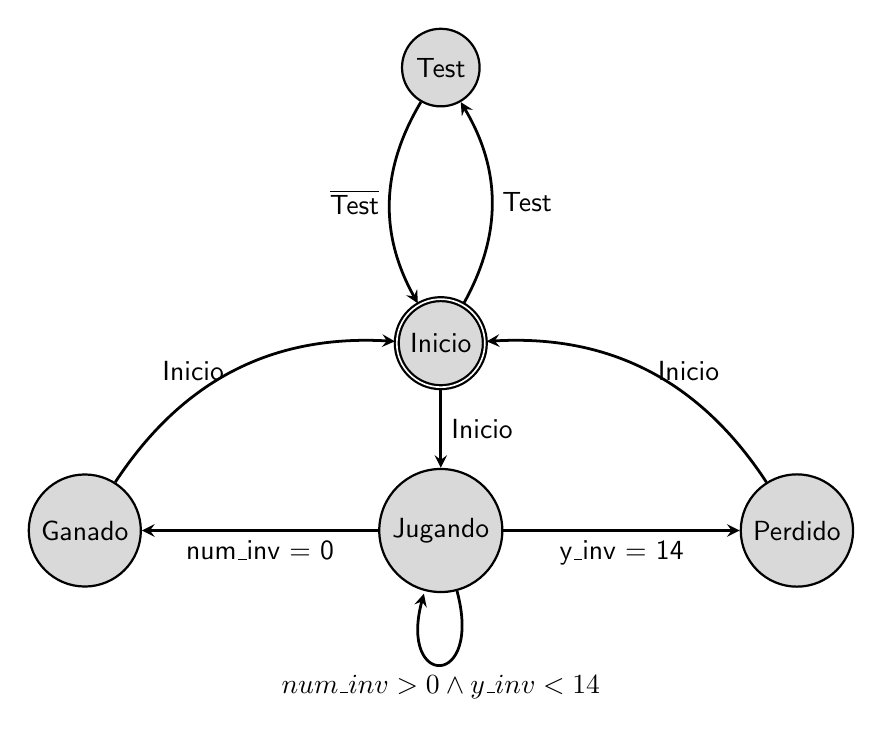
\begin{tikzpicture}[->,  % makes the edges directed
  >=stealth, % makes the arrow heads bold
  node distance=3.5cm, % specifies the minimum distance between two nodes. Change if necessary.
  every state/.style={thick, fill=gray!30}, % sets the properties for each ’state’ node
  initial text=$ $, % sets the text that appears on the start arrow]
]
    \node[state, accepting] (1) {Inicio};
    \node[state, above of=1] (2) {Test};
    \node[state, below=1cm and 1cm of 1] (3) {Jugando};
    \node[state, left=2cm and 3cm of 3] (4) {Ganado};
    \node[state, right=2cm and 3cm of 3] (5) {Perdido};

    \draw[->,line width=1pt] (1) edge[right, bend right] node{Test} (2)
    (2) edge[left, bend right] node{$\overline{\text{Test}}$} (1)
    (1) edge[right] node{Inicio} (3)
    (3) edge[below] node{num\_inv = 0} (4)
    (3) edge[below] node{y\_inv = 14} (5)
    (4) edge[left, bend left] node{Inicio} (1)
    (5) edge[right, bend right] node{Inicio} (1)
    (3) edge[loop below] node{$num\_inv > 0 \wedge y\_inv < 14$}(3);
    (5) edge[loop right] (5);
  \end{tikzpicture}
  
  \caption{Maquina de estados del juego}
  \label{fig:statemachine}
\end{figure}

\begin{itemize}
  \item \textcolor{dred}{Test}: En este estado se muestra un patron de ajedrez de 20$\times$15. Se entra en el estado cuando se pulsa en boton \textbf{Test} y se sale cuando se suelta el botón
\end{itemize}

\section{Implementación}
\section{Recursos utilizados}

\end{document}
